\chapter{Experimente} \label{chap:experimentresult}

Anknüpfend an das vierte Kapitel listet das fünfte Kapitel zunächst die Rahmenbedingungen des Trainings der EfficientNet-Modelle und die Metriken zur Evaluation auf. Danach wird die Leistung der EfficientNet-Modelle auf den zugeteilten Testdatensätzen beschrieben. Das Kapitel wird mit einer Diskussion über die Auswahl des besten trainierten Modells zur Tierklassifizierung abgeschlossen.

Hier ist zu beachten, dass eine Inspektion der Leistung des MegaDetectors auf den gecrawlten Datensätzen nicht durchgeführt wurde. Der Grund dafür ist, dass iNat sowie Nat4\&WCS über keine Ground-Truth Bounding Boxes zum Vergleich mit den ausgegebenen MegaDetections verfügen. Daher ist es nicht möglich, die Leistung des Gesamtmodells zur Tierarterkennung zu ermitteln. Ein möglicher Lösungsansatz zu diesem Problem wird in \autoref{sec:ausblick} vorgestellt.

\section{Trainingskonfigurationen}

In diesem Abschnitt werden die zum Training verwendeten Hardware und Hyperparameter aufgeführt.

\subsection{Verwendete Hardware}

Zum Training wurde ein mit einer GPU vom Typ \emph{NVIDIA GeForce GTX TITAN X} ausgestatteter Computer verwendet. Diese Grafikkarte verfügt über einen 12GB GDDR5-\emph{Speicher}, eine \emph{Compute Capability} von 5.2 und 3072 \emph{CUDA-Kerne} \cite{gtxtitanx}. Diese Spezifikationen lassen sich wie folgt verstehen.

\begin{description}
	\item[Speicherkapazität]

	Das Training eines CNN-Modells erfordert enormen Speicherplatz, weil der Backward Pass des Backpropagation-Algorithmus alle während des Forward Pass berechneten Zwischenwerte benötigt. Je höher die Speicherkapazität einer Grafikkarte ist, desto mehr Zwischenvariablen können gespeichert werden, was das Training von komplexeren CNN-Modellen ermöglicht.
	
	\item[Compute Capability] 
	
	Unter Compute Capability versteht man eine Versionsnummer, die die von der GPU-Hardware unterstützten Funktionen identifiziert. Je höher die Compute Capability ist, desto neuer und fortschrittlicher sind die unterstützten Funktionen, was zu höherer Rechenleistung der Grafikkarte führt. Dadurch verkürzt sich die Trainingsdauer.
	
	\item[CUDA-Kerne] 
	
	Die CUDA-Kerne einer NVIDIA-Grafikkarte sind für die Parallelverarbeitung zahlreicher komplexer Berechnungen optimiert. Je höher die Anzahl von CUDA-Kernen in einer Grafikkarte ist, desto mehr Berechnungen können parallel verarbeitet werden und somit kürzer dauert das Training.
\end{description}

Um die Qualität der GPU GeForce GTX TITAN X genauer einzuschätzen, kann man zum Vergleich die GPU NVIDIA GeForce GTX 580 heranziehen, mit der das in \autoref{subsec:milestonecnn} erwähnte CNN-Modell AlexNet trainiert wurde. Diese Grafikkarte verfügt über einen 1,5GB GDDR5-Speicher, eine \emph{Compute Capability} von 2.0 und 512 \emph{CUDA-Kerne} \cite{gtx580}. Laut der Autoren von AlexNet dauerte das Training von diesem CNN-Modell auf zwei GeForce GTX 580 GPUs fünf bis sechs Tage \cite[7]{10.1145/3065386}.

\subsection{Verwendete Hyperparameter}

Die Hyperparameter zur Steuerung des Trainingsprozesses wurden wie folgt gesetzt.
%Aber 

\begin{itemize}
	\item $\textbf{Batch-Größe} = 16$. 
	
	Da der Out-Of-Memory-Error bereits während des Trainings des B4-Modells mit einer Batch-Größe von 32 auftrat, wurde dieser Hyperparameter auf 16 festgelegt.
	
	\item $\textbf{Lernrate (Transfer Learning)} = 10^{-3}$. 
	
	In der Implementierung wurde zur Optimierung der Gewichte der zu trainierenden EfficientNet-Modelle der Optimizer \emph{Adam}\footfullcite{KerasAdam} benutzt. Dabei ist der Standardwert für die Lernrate $10^{-3}$.
	
	\item $\textbf{Lernrate (Feintuning)} = 10^{-4}$. 
	
	Die Lernrate zum Feintuning wurde zur Vermeidung von Overfitting auf den kleinen Wert von $10^{-4}$ eingestellt.
	
	\item $\textbf{Anzahl der Trainingsepochen (Transfer Learning)} = 25$. 
	
	In der Regel gibt es keinen Standardwert für die Anzahl der Trainingsepochen. Der Wert $25$ kommt von einer Beispielimplementierung eines EfficientNet-Modells nach dem Transfer-Learning-Konzept zur Klassifizierung von 120 Hunderassen\footfullcite{EffNetEpochNumb} .
	
	\item $\textbf{Anzahl der Trainingsepochen (Feintuning)} = 75$. 
	
	Da die Lernrate zum Feintuning klein ausgewählt wird, muss sichergestellt werden, dass es zur Bestimmung der optimalen Gewichte hinreichende Trainingsepochen gibt. Dazu wird die Anzahl der Trainingsepochen beim Feintuning dreimal so groß wie die Epochanzahl beim Transfer Learning abgeschätzt, also auf $75$ gesetzt.
\end{itemize}

\section{Bewertungsmetriken} \label{sec:evalmetrics}

Für die Leistungsbewertung der trainierten EfficientNet-Modelle kommen die Top-1, Top-5 Accuracy sowie \emph{Mean Average Precision} (abgekürzt: mAP) zum Einsatz.

\begin{description}
	\item[Top-1 \& Top-5 Accuracy] Die Accuracy lässt sich wie folgt kalkulieren.
	
	\begin{equation} \label{eq:accuracy}
		\text{Accuracy} = \frac{\text{Anzahl korrekt klassifizierter Bilder}}{\text{Gesamtzahl von Bildern}}
	\end{equation}
	
	Bei der Top-1 Accuracy gilt ein Bild als korrekt klassifiziert, wenn das Modell die Klasse dieses Bilds genau vorhersagt. Bei der Top-5 Accuracy zählt ein Bild als korrekt klassifiziert, wenn sich die richtige Klasse in den wahrscheinlichsten fünf Klassen befindet, die das Modell für dieses Bild vorhersagt. Sowohl die Top-1 als auch die Top-5 Accuracy sind Standardmetriken zur Leistungsmessung im Bereich der Bildklassifizierung. Allerdings sind diese beiden nicht in der Lage, Modelle zu erkennen, die vom Imbalanced-Classification-Problem befallen sind. Ein solches Modell kann dennoch eine hohe Top-1 bzw. Top-5 Accuracy erreichen, insbesondere wenn die Testdatensätze unausgewogen sind.
	
	\item[mAP] Die Formel zur Berechnung der mAP ist
	
	\begin{equation} \label{eq:map}
		\text{mAP} = \frac{1}{\lvert K\rvert}\sum_{k \in K}AP(k)
	\end{equation}
	
	wobei $K$ die Menge der Klassen ist und $AP(k)$ sich auf die \emph{Average Precision} (AP) der Klasse $k$ bezieht. Die AP misst, wie gut das Modell für eine Klasse funktioniert, d.~h. wie präzise seine vorhergesagten Wahrscheinlichkeiten bezüglich dieser Klasse sind (für alle Testbilder). Der Vorteil von der mAP besteht darin, dass diese Metrik für die Erkennung der Modelle geeignet ist, die vom Imbalanced-Classification-Problem beeinflusst werden: Der mAP-Wert eines Modells ist nur hoch, wenn die APs aller oder der meisten Klassen gleichzeitig hoch sind, d.~h. wenn das Modell für (fast) alle Klassen gut funktioniert. Die mAP ist also weniger anfällig gegenüber unausgewogenen Testdatensätzen als die Top-1 bzw. Top-5 Accuracy.
	
	%\item[MegaCertainty] Die MegaCertainty kann durch folgende Formel berechnet werden:
	
	%\begin{equation} \label{eq:MegaCertainty}
	%	\text{MegaCertainty} = \frac{\text{Anzahl von MegaDetections mit Confidence-Wert} \geq 0,8}{\text{Gesamtzahl von Tierbildern}}
	%\end{equation}

%	. Jedoch kann man zur Evaluierung des MegaDetectors die MegaCertainty als Abschätzung für die Accuracy benutzen. Grundsätzlich stellt die MegaCertainty den Anteil der Tierbilder dar, deren Tiere vom MegaDetector mit großer Sicherheit lokalisiert werden können. Wenn angenommen wird, dass sich aus jedem Bild nur eine MegaDetection ergibt und alle MegaDetections mit Confidence-Werten über 0,8 zuverlässig sind, dann kann mit MegaCertainty gemessen werden, wie gut der MegaDetector für eine vorgegebene Menge von Tierbildern funktioniert (ob der MegaDetector die Tiere darin gut lokalisiert oder nicht). Auf diese Weise kann die MegaCertainty auch zur Leistungsabschätzung des Gesamtmodells dienen, das zur Tierarterkennung im Rahmen dieser Arbeit entwickelt wird. Die Abschätzung erfolgt durch die Multiplikation der MegaCertainty, die aus der Anwendung des MegaDetectors auf die gecrawlten Datensätze resultiert, mit der Test-Top-1 Accuracy des EfficientNet-Modells, das zur Tierklassifizierung ausgewählt wird.
	

	
\end{description}

%Es ist auch wichtig zu nennen, dass für die Umsetzung der obigen Bewertungsmetriken die richtigen Implementierungen in der dazu verwendeten API ausgewählt werden müssen, sonst kommt es zur falschen Evaluierung der Modelle, was tatsächlich während des Trainings geschah. Im Rahmen dieser Arbeit wurde für die Umsetzung der Bewertungsmetriken die \emph{Tensorflow-API}\footfullcite{TFmetric} verwendet, in der es zwischen \code{CategoricalAccuracy} und \code{SparseCategoricalAccuracy} unterschieden wird. Beide Implementierungen dienen zur Messung der Top-1 Accuracy, jedoch wurde nur letztere benutzt, weil beim Importieren der Datensätze die Labels der Trainingsbilder (wissenschaftliche Namen der Tierarten) \emph{Integer-kodiert} waren. Erstere kommt nur zum Einsatz, wenn die Labels \emph{One-hot-kodiert} sind. Mehr Informationen über die Kodierung der Labels lassen sich in \cite{CateEncode} finden.

\section{Ergebnisse}

\autoref{table:results} stellt die erzielten Testergebnisse der trainierten EfficientNet-Modelle dar. Dabei sind drei Punkte zu beachten.

\begin{table}[!h]
	\centering
	\caption{Leistung der trainierten EfficientNet-Modelle auf beiden Testdatensätzen von iNat und Nat4\&WCS zusammen sowie auf dem einzelnen Testdatensatz von Nat4\&WCS}
	\label{table:results}
	\begin{tabular}{>{\centering}m{0.5cm}|>{\raggedright}m{1.8cm}|>{\centering}m{1.3cm}>{\centering}m{1.3cm}c|>{\centering}m{1.3cm}>{\centering}m{1.3cm}c}
		\multicolumn{2}{c|}{\textbf{Eff.Net-Modell}}            & \multicolumn{3}{c|}{\textbf{Getestet auf beiden}}          & \multicolumn{3}{c}{\textbf{Getestet auf Nat4\&WCS}}                 \\
		\hline
		\textbf{ID} & \textbf{Trainiert auf} & \textbf{Top-1 Acc. (\%)} & \textbf{Top-5 Acc. (\%)} & \textbf{mAP (\%)} & \textbf{Top-1 Acc. (\%)} & \textbf{Top-5 Acc. (\%)} & \textbf{mAP (\%)} \\
		\hline
		\multirow{3}{*}{B3}   & Beiden     & 92,4               & 98,9               & 95,2        & 92,6               & 99,0               & 91,8        \\
		%\cline{2-8}
		& iNat                   & 60,8               & 82,4               & 68,7        & 46,7               & 75,7               & 46,2        \\
		%\cline{2-8}
		& Nat4\&WCS              & 80,8               & 94,9               & 79,2        & 93,6               & 99,2               & 94,1        \\
		\hline
		\multirow{3}{*}{\textbf{B4}}   & \textbf{Beiden}     & \textbf{92,9}               & \textbf{98,6}               & \textbf{96,0}        & \textbf{92,7}               & \textbf{99,0}               & \textbf{93,9}        \\
		%\cline{2-8}
		& iNat                   & 64,1               & 83,2               & 71,3        & 51,1               & 77,0               & 52,6        \\
		%\cline{2-8}
		& Nat4\&WCS              & 79,5               & 93,9               & 81,5        & 93,1               & 99,0               & 94,4        \\
		\hline
		B5                    & Beiden     & 92,1               & 98,6               & 94,9        & 92,0               & 99,0               & 92,1  \\
		\hline     
	\end{tabular}
\end{table}

\begin{itemize}
	\item Es wurden auch EfficientNet-Modelle getestet, die zuvor nur auf iNat oder Nat4\&WCS trainiert worden waren. Dieses Testen dient zur Untersuchung der Frage, ob es tatsächlich nötig ist, Modelle sowohl mit hochwertigen NK-Bildern als auch mit Kamerafallenbildern zu trainieren. Wenn zum Training lediglich ein Bildertyp benötigt wird, kann man die restlichen potenziellen Modelle einfach mit entweder iNat oder Nat4\&WCS trainieren, um Zeit und Ressourcen zu sparen.
	
	\item Die trainierten EfficientNet-Modelle wurden zusätzlich auf dem Testdatensatz von Nat4\&WCS getestet, um zu prüfen, wie gut diese Modelle mit nur Kamerafallenbildern funktionieren, insbesondere wenn die Bilder von Natur4.0 ausschließlich von Kamerafallen aufgenommen werden.
	
	\item Das Trainingsverfahren wurde nach dem Training des B5-Modells (auf dem gesamten Trainingsdatensatz) gestoppt, weil bereits zu diesem Zeitpunkt ersichtlich war, welches von den trainierten Modellen das Optimale zur visuellen Erkennung von Tierarten im Projekt Natur 4.0 ist (Mehr dazu in \autoref{sec:discussion}).
\end{itemize}

\section{Diskussion} \label{sec:discussion}

Aus \autoref{table:results} lassen sich folgende bedeutsame Schlussfolgerungen ziehen.

\begin{itemize}	
	\item Wie es erwartet wurde, funktionieren die EfficientNet-Modelle, die nur auf iNat trainiert wurden, nicht gut auf Testdatensätzen, die auch Kamerafallenbilder enthalten. Daher empfiehlt es sich, Modelle nicht nur mit hochwertigen NK-Bildern, sondern auch mit Kamerafallenbildern zu trainieren. 
	
	\item Aus der Tabelle geht hervor, dass es am besten ist, die nur auf Kamerafallenbildern (Nat4\&WCS) trainierten EfficientNet-Modelle zur Tierklassifizierung einzusetzen, denn solche Modelle erzielten die höchste Leistung in allen drei Bewertungsmetriken beim Nat4\&WCS-Testdatensatz und letztlich sind die im Rahmen des Projekts Natur 4.0 zu klassifizierenden Bilder Kamerafallenbilder. Jedoch ist dieser Einsatz im Rahmen dieser Arbeit nicht empfehlenswert. Es kann vom Projekt Natur 4.0 gefordert werden, dass das zur Tierklassifizierung ausgewählte Modell auch in der Lage sein muss, NK-Bilder zu klassifizieren, damit neben der visuellen Tierarterkennung weitere Zwecke im Rahmen oder außerhalb des Projekts erfüllt werden können. Ein weiterer Grund, EfficientNet-Modelle auch auf NK-Bildern zu trainieren, ist, dass es für einige Klassen (zu erkennende Tierarten im Rahmen des Projekts Natur 4.0) fast keine Kamerafallenbilder gibt. Außerdem ist der Leistungsunterschied zwischen Modellen, die auf beiden Bildertypen trainiert wurden, und solchen, die nur aus Kamerafallenbildern lernten, beim Testdatensatz von Nat4\&WCS geringfügig. Auf lange Sicht bieten die Ersteren im Gegenzug für marginalen Leistungsabfall mehr potenzielle Anwendungen als die Letzteren.
	
	\item Die auf beiden Bildertypen trainierten EfficientNet-Modelle konnten auch gute Leistung (mindestens 91\% in allen drei Bewertungsmetriken) beim Nat4\&WCS-Testdatensatz erreichen. Damit wird sichergestellt, dass diese Modelle zur visuellen Tierarterkennung im Projekt Natur 4.0 einsetzbar sind. \textbf{In Bezug auf die Gesamtleistung ist B4 das beste trainierte EfficientNet-Modell für die Tierklassifizierung (im Rahmen dieser Arbeit)}. Dieses Modell liefert die höchste Top-1 Accuracy sowie mAP (92,9\% bzw. 96,0\%) für den vollständigen Testdatensatz (iNat und Nat4\&WCS).
	
	
\end{itemize}

Man kann dennoch argumentieren, dass B6 und B7, obwohl sie im Rahmen dieser Arbeit nicht trainiert wurden, aufgrund von \autoref{table:effnetaccu} viel bessere Leistung als B4 erzielen können und daher trainiert werden sollen. Dieses Argument lässt sich aber durch Schlussfolgerungen aus \autoref{fig:EffNetModelCompare} widerlegen. \autoref{fig:EffNetModelCompare} zeigt den Verlauf der während des Trainings aufgezeichneten Validierung-Top-1, -Top-5 Accuracy sowie -mAP von den EfficientNet-Modellen B3, B4 und B5. Daraus lässt sich abschätzen, dass ab B5 die EfficientNet-Modelle dazu tendieren, eine niedrigere Leistung zu erreichen. Dies kann daran liegen, dass die größeren Modelle von B5 bis B7 über viel mehr Parameter als nötig verfügen, was zu Overfitting führt. Es ist auch nicht sinnvoll, B6 und B7 zu trainieren, weil aus \autoref{fig:EffNetModelCompare} abgeleitet werden kann, dass sich die Trainingsdauer mit jedem nachfolgenden größeren EfficientNet-Modell verdoppelt. Dies bedeutet, dass das Training von B6 und B7 bis zu 120 bzw. 240 Stunden dauern kann, was im Vergleich zu B4 extrem lang ist, während die dadurch erzielte Leistung niedriger als die von B4 sein kann.

\begin{figure}[h]
	\centering
	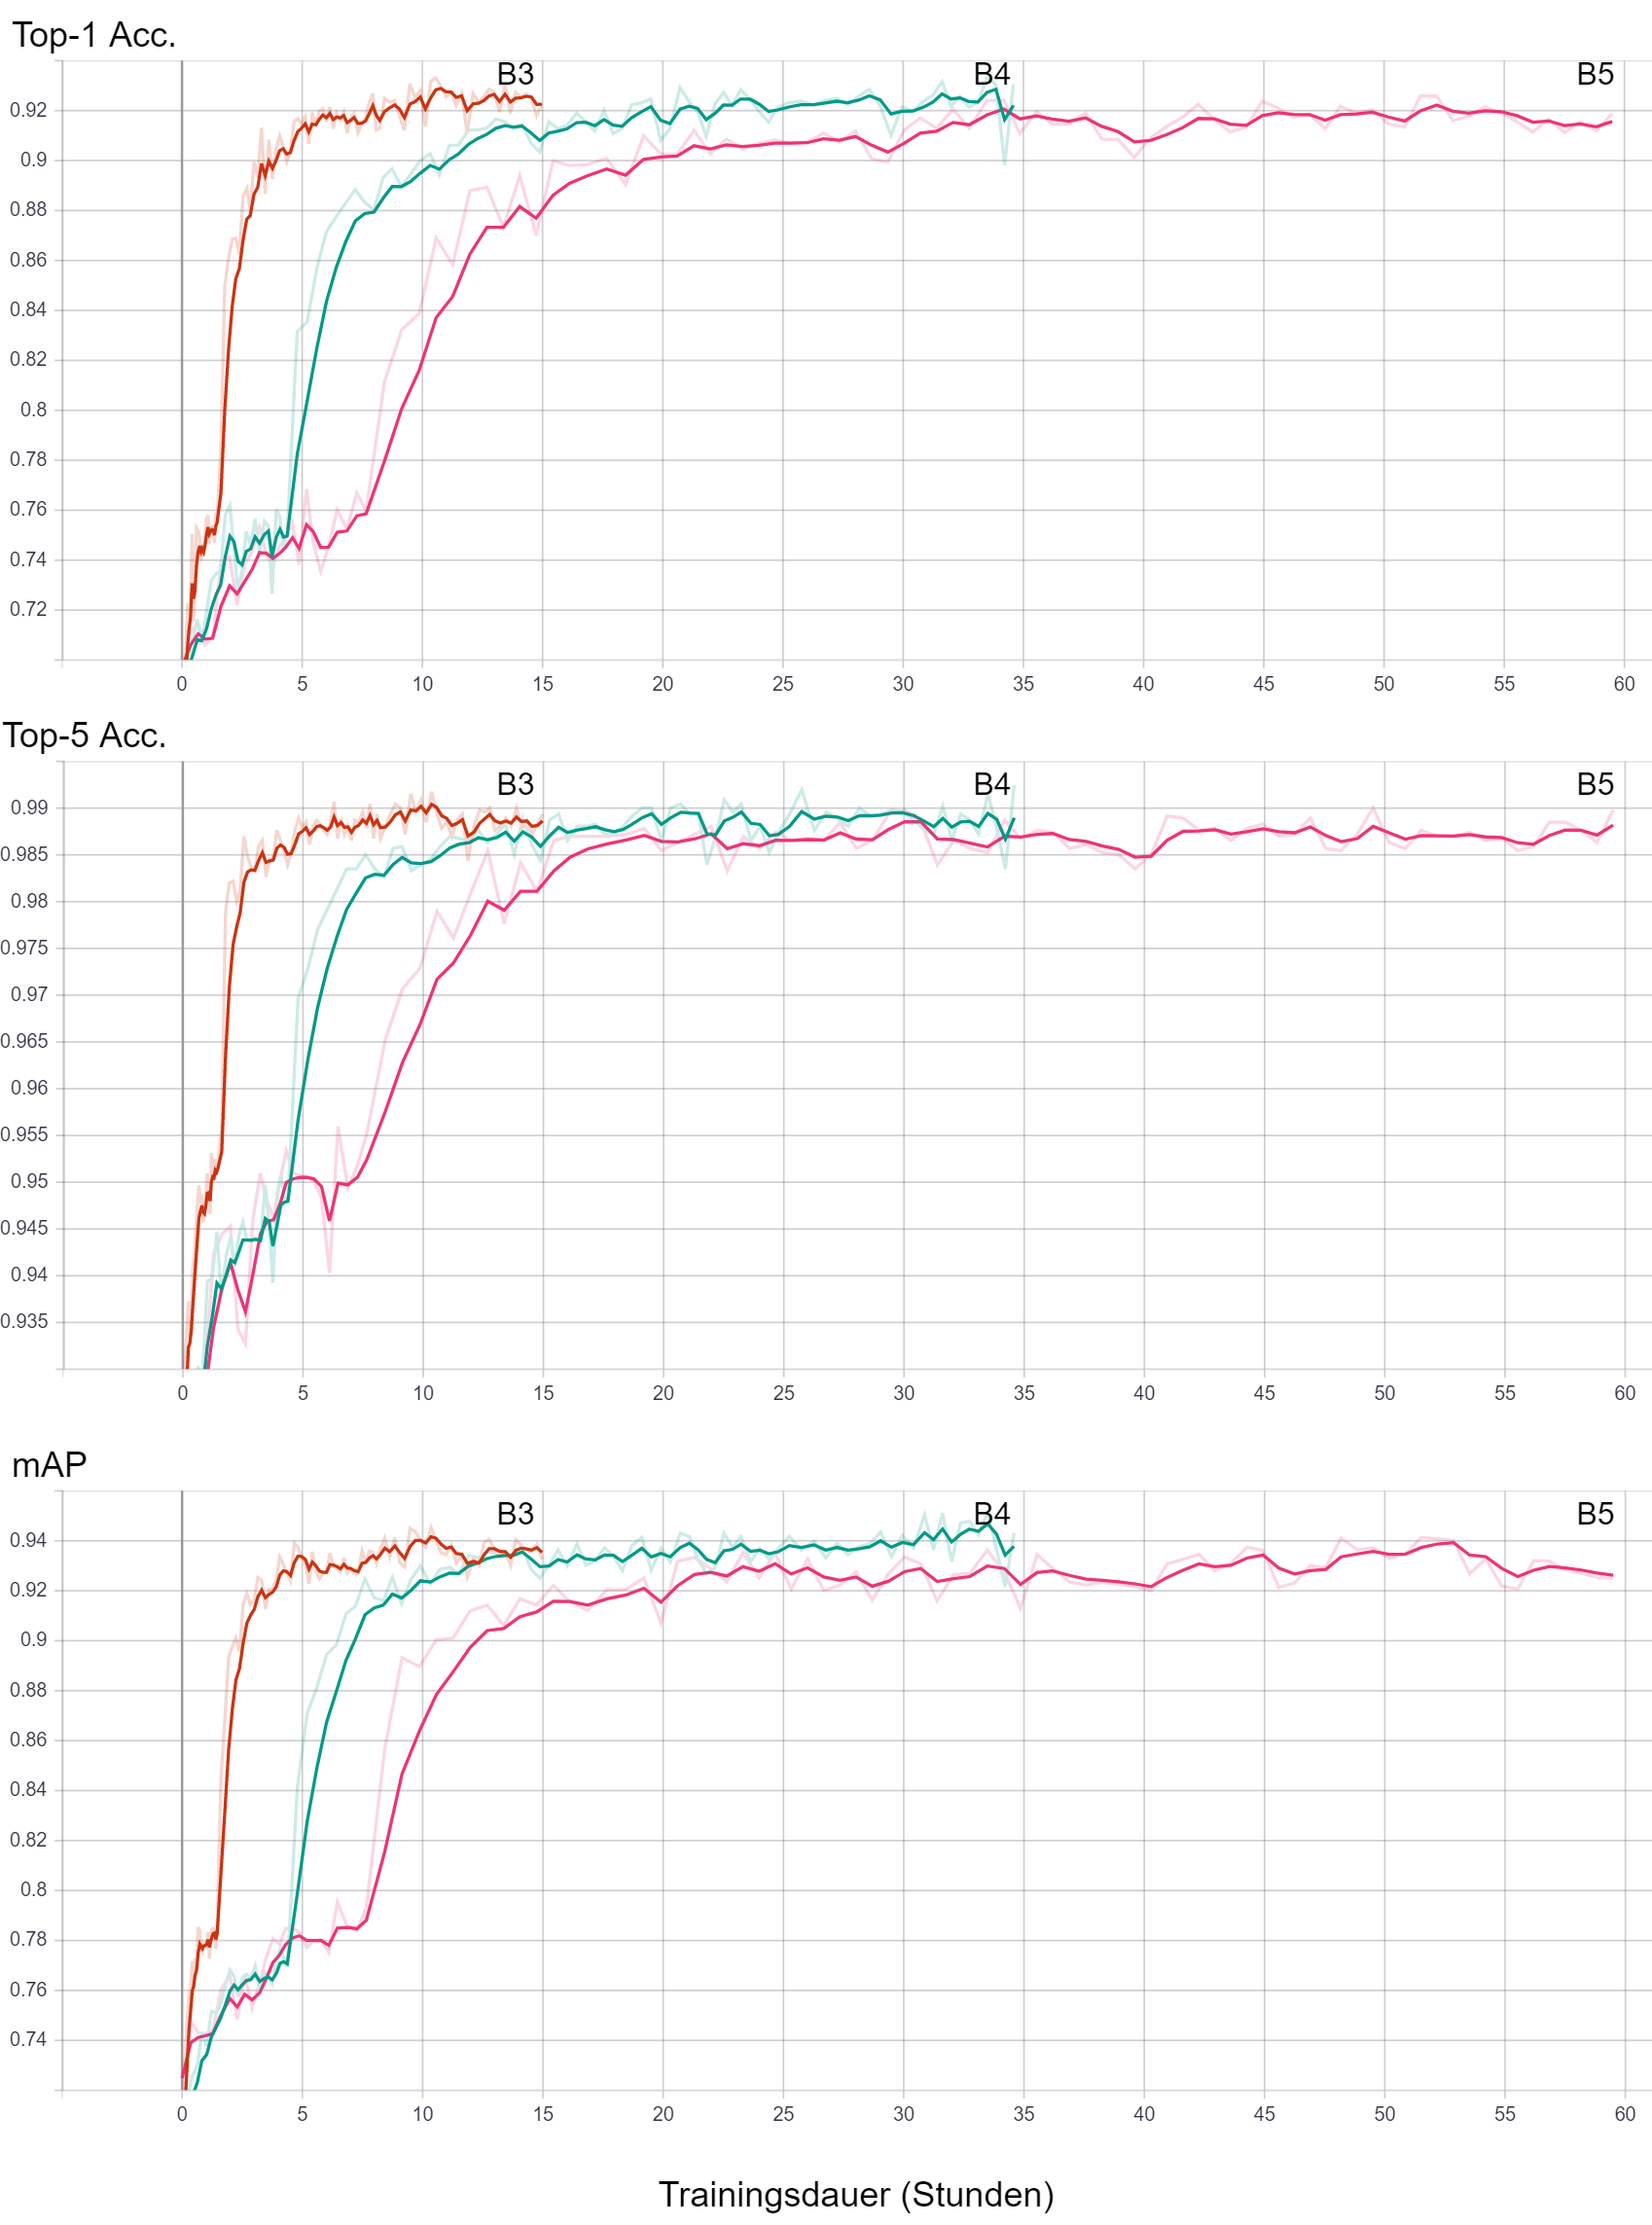
\includegraphics[width=\linewidth]{images/EffNetModelCompare}
	\caption{Leistung auf dem gesamten Validierungsdatensatz während des Trainings von den EfficientNet-Modellen B3, B4 und B5, die sowohl mit iNat als auch mit Nat4\&WCS trainiert wurden}
	\label{fig:EffNetModelCompare}
\end{figure}


